%===================================== CHAP 2 =================================
\cleardoublepage

\chapter{Background}

To understand what sets our system apart from other standard search engines, its important to understand how CBR works. This chapter elaborates how CBR works, what recommendation systems are, and what MyCBR is; the tool which was used to implement CBR in Utsida.



\section{Case-based Reasoning}
Case-Based Reasoning (CBR) is a methodology in AI for solving problems, and is essentially based on experience. This experience can be used to solve a large range of problems, including complex combinatorial problems, or yield solutions where uncertainty is involved. Implied by the name, CBR can be broken down into two main concepts; \textit{cases} and \textit{reasoning}.

\begin{enumerate}
    \item Case: An experience of a solved problem, usually represented as a feature vector (see 2.1.1). A case consists of two parts: a problem description and a solution to the problem. A Case-Based Reasoning System (CBRS) stores all of its cases in a \textit{Case Base}.
    \item Reasoning: The approach of drawing conclusions using cases, given a problem to be solved.
\end{enumerate}

Reasoning in CBR differs from other kinds of reasoning because it does not lead from true assumptions to true conclusions. This means that for two cases with identical problem descriptions, the solution to one of them might not be the solution for the other. The recorded experience in the first case may not be exactly similar to the other case. To be reused, it only has to be \enquote{similar}.

\subsection{Feature Vectors}
A case is usually represented as a feature vector, consisting of a few to many pairs of attributes and their values. A common example is the diagnosis of a sick patient, where a collection of symptoms and weather the patient has them is the problem description, and the final diagnoses is the solution to the case, as illustrated by the following diagram.


\begin{table}[H]
\centering
\caption{Classic case representation with attribute-value pairs for the problem description and the solution.}
\label{my-label}
\begin{tabular}{|l|l|}
\hline
\rowcolor[HTML]{C0C0C0} 
Attribute           & Value     \\ \hline
Nausea              & Yes       \\ \hline
Fever               & Yes       \\ \hline
Malaise             & Dizzy     \\ \hline
Blood pressure      & Normal    \\ \hline
Vision changes      & No        \\ \hline
Shortness of breath & No        \\ \hline
Diagnosis           & Influensa \\ \hline
\end{tabular}
\end{table}

\subsection{The CBR-Cycle}

Aamodt & Plaza\cite{aamodt1994case} defined a model which explain the problem solving cycle in CBR, as shown by the diagram below. 

\begin{figure}[H]
    \centering
    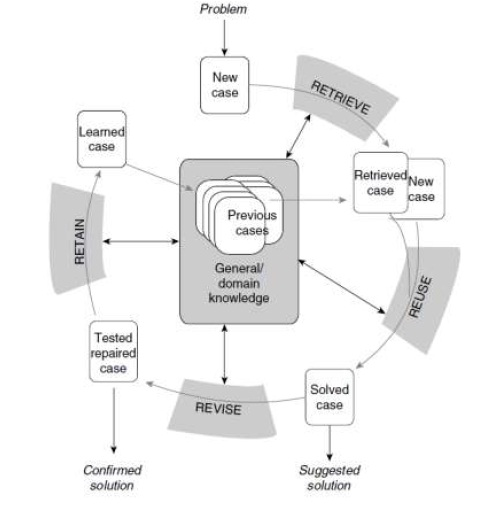
\includegraphics[width=0.5\textwidth]{fig/cbr_cycle.jpg}
    \caption{The CBR Cycle}
    \label{fig:cbr_cycle}
\end{figure}

The cycle defines four distinct processes which a case goes through:

\begin{description}
\item [Retrieve:] The most similar case is retrieved from the system's case base, so that it can be compared to a new case.
\item [Reuse:] The solution to the retrieved case is applied to the new case.
\item [Revise:] Confirms that the proposed solution solves the new case, or if its no applicable.
\item [Retain:] Retains the new case with the given solution in the case base for future usage.
\end{description}

\subsection{Similarity Measures}






\section{Reccomender Systems}
Recommender systems are used extensively in both research and commercial products. These systems provide several possible solutions that might be viable for the user to choose. Several published research papers have explored different approaches to recommender systems \cite{mulyana2015case}\cite{quijano2011happy} \cite{}.

case-based reccommender systems use CBR as



\section{MyCBR}
MyCBR is a tool for rapid prototyping of CBR systems with focus on similarity-based retrieval step \cite{MyCBR}. It was used extensively throughout the project to assist with both prototyping and in system production. MyCBR is divided in two main parts, the workbench and the SDK. 


\subsection{SDK}
The MyCBR SDK provides a access point for implementing the functionality of myCBR in a custom application. 


\subsection{Workbench}


\cleardoublepage